\documentclass[oneside,a4paper,12pt]{article} % Gibt das Seitenformat und die Schriftgröße an.

% -------------------------------------- Integration von Packages -------------------------------------- 
% Literatur und Sprache
	\usepackage[ngerman]{babel}
	\usepackage[style=bwl-FU,backend=bibtex,natbib=true,maxcitenames=2]{biblatex}
	\addbibresource{Content/Literaturverzeichnis.bib}
	
% Format und Seitenlayout
	\usepackage[left=3cm,right=3cm,bottom=3cm]{geometry} % Legt die linken und rechten Seitenränder fest.
	\usepackage{setspace} % Paket, das die Änderung des Zeilenabstands ermöglicht.
	\setstretch{1.3} % Legt einen Zeilenabstand von 1,3 fest.
	\parindent0pt % Definition des Einrückens bei neuem Abschnitt.
    \parskip10pt % Definition des Abstands zweier Absätze.
	\usepackage{footmisc} % Implementiert eine Reihe von Fußnotenoptionen.
	\renewcommand{\footnotelayout}{\setstretch{1}} % Legt einen Zeilenabstand von 1 für die Fußnoten fest.
	\pagestyle{headings} % Erzeugt eine Überschrift mit der Seitenzahl und der Überschrift des aktuellen Abschnitts.
	\usepackage[utf8]{inputenc} % Ermöglicht die Verwendung von Sonderzeichen.
	\usepackage[T1]{fontenc} % Ermöglicht die Verwendung von Sonderzeichen.
	\usepackage{eurosym} % Einbindung von €
	\usepackage{acronym} % Ermöglicht die Einbindung eines Abkürzungsverzeichnisses.
	\usepackage{nomencl} % Nützlich, um eine Liste von Symbolen zu erstellen.
	\usepackage{enumerate} % Nützlich für Auflistungen.
	\usepackage{color} % Ermöglicht die Definition von Farben.
	
% Tabellen und Graphiken
	\usepackage{booktabs} % Verbessert das Design der Tabellen
	\usepackage{longtable} % Erlaubt Tabellen, die länger als eine Seite sind.
	\usepackage{multirow,multicol} % Mit diesen Paket ist es nun möglich, Spalten und Zeilen innerhalb von Tabellen zu kombinieren.
	\usepackage{graphicx} % Ermöglicht die Implementierung von Grafiken.
	\usepackage{subfig} % Ermöglicht eine Abbildung aus mehreren Unterabbildung.
	\graphicspath{{./Graphs/}} % Sagt LATEX, dass die Bilder in einem Ordner namens 'Graphs' unter dem Verzeichnis des Hauptdokuments gespeichert werden.
	\usepackage[hypcap=false]{caption} % Bietet viele Möglichkeiten zur Anpassung der Beschriftungen.	

% Mathematik
	\usepackage{amscd,amsfonts,amsmath,amssymb,amsthm,amscd,bbm} % Erweitert das Mathematikset.


% -------------------------------- Informationen der Arbeit -------------------------------- 
% Bitte geben Sie diese Informationen zu Beginn einmal an. Auf diese Weise werden die Lücken im Folgenden automatisch ausgefüllt.
	\newcommand{\name}{Finn Vincent Drexhage} % Geben Sie Ihren Namen an.
	\newcommand{\dateofthesis}{16. Juni 2025} % Geben Sie das Datum der Einreichung Ihrer Arbeit an.
	\newcommand{\titleofthesis}{Hedging Renenwables with Location Spreads} % Geben Sie den Titel Ihrer Arbeit an.
	\newcommand{\streetadress}{Ruhesteinstraße 5} % Geben Sie Ihre Adresse an.
	\newcommand{\postalcode}{71083} % Geben Sie Ihre Postleitzahl an.
	\newcommand{\city}{Herrenberg} % Geben Sie Ihre Stadt an.
	\newcommand{\email}{uvyta@student.kit.edu} % Geben Sie Ihre E-Mail Adresse an.
	\newcommand{\typeofthesis}{Bachelorarbeit} % Geben Sie die Art der Arbeit an: Seminararbeit, Bachelorarbeit, Masterarbeit.

% --------------------------------- Definition of hyperlinks --------------------------------- 
% Hyperreferenzen
	\usepackage{hyperref}
	\definecolor{darkblue}{rgb}{0,0,.5}
	\hypersetup{
	    pdfstartview={FitH}, 
        colorlinks=true,
        linkcolor=black,
        citecolor=darkblue,
        urlcolor=black,
        pdftitle=\titleofthesis,
        pdfsubject=\typeofthesis,
        pdfauthor=\name,
        bookmarksopen
        }
        







% ----------------------------------- Start des Dokuments ----------------------------------- 	
\begin{document}
	\setcounter{page}{2} % Umschlagseiten und Titelseite sind nicht nummeriert. Die Nummerierung beginnt auf Seite 2.
	
% Titelseite 
	\newgeometry{left=3cm, right=3cm, bottom=2cm}
\begin{titlepage}
		\begin{center}
			{\Large Karlsruher Institut für Technologie \\
			\vspace{0.6cm}
			Institut für Finanzwirtschaft, Banken und Versicherungen\\
			Abteilung Financial Engineering und Derivate\\
			Prof. Dr. Marliese Uhrig-Homburg} \\[4.5cm]
			{\large{\typeofthesis}} \\[1.7cm]
			\setstretch{20.0}
			{\Huge {\titleofthesis}}
			\setstretch{1.3} \\[6cm]
		\end{center}
				
		\begin{tabular}{ll}
        Autor: 	    & {\name}\\
                    & {\streetadress}\\
                    & {\postalcode} {\city}\\
					& E-Mail: {\email}\\\\
        Karlsruhe, & {\dateofthesis}\\
    	\end{tabular}
\end{titlepage}
\restoregeometry 

% Inhaltsverzeichnis
	\setcounter{page}{1}\renewcommand{\thepage}{\roman{page}} % Setzt die Nummerierung auf römisch klein.
	\newpage 
	\tableofcontents % Erzeugt Inhaltsverzeichnis.

% Abbildungsverzeichnis 
	\newpage
	\listoffigures % Fügt das Abbildungsverzeichnis ein.
	\addcontentsline{toc}{section}{Abbildungsverzeichnis} % Fügt das Abbildungsverzeichnis dem Inhaltsverzeichnis hinzu.
		
% Tabellenverzeichnis (auskommentieren, wenn keine Tabellen in der Arbeit vorhanden sind).
	\newpage
	\listoftables % Fügt das Tabellenverzeichnis ein.
	\addcontentsline{toc}{section}{Tabellenverzeichnis} % Fügt das Tabellenverzeichnis dem Inhaltsverzeichnis hinzu.
	
% Hauptteil der Arbeit 
    \newpage
	\setcounter{page}{1}\renewcommand{\thepage}{\arabic{page}} % Setzt die Nummerierung auf arabisch.
	\section{Motivation}
\label{sec:Motivation}

\begin{itemize}
    \item Einfluss der Attraktivität des Strommarktes auf Investoren und Energiewende \textbf{8}
    \item Ziele der EU für Marktkopplung \textbf{19}
    \item Problem Preisspread für EE Herstellerrelevant \textbf{1, 2}
    \item Ziel ist Absicherung von Herstellern gegen Preisspread Risiken \textbf{1, 2, 8}
    \item Ansatz ist statistische Muster finden und dann ausnutzen mit Hedging-Produkten
    \item Kurze Zusammenfassung der Ergebnisse der Arbeit
\end{itemize}
	\section{Grundlagen zu Location Spreads}
\label{sec:Grundlagen zu Location Spreads}

isudgbesiade

\subsection{Funktionsweise des Strommarktes}
\label{sec:Funktionsweise des Strommarktes}
Der europäische Strommarkt ist ein stark integriertes System mit vielen einzelnen Akteuren, die eng zusammenarbeiten und für den grenzüberschreitenden Handel eine große Rolle spielen. Ein wesentliches Element dieser Marktarchitektur ist die Aufteilung in verschiedene Preiszonen. Häufig entsprechen Preiszonen den Grenzen der Länder, wobei es hiervon Ausnahmen gibt, wie Deutschland und Luxemburg, die eine Zone bilden, und die skandinavischen Länder, die jeweils in mehrere Zonen unterteilt sind. Innerhalb einer Preiszone herrscht überall der gleiche Strompreis trotz teilweise verschiedener Netzbedingungen\footnote{So wird beispielsweise seit einiger Zeit diskutiert, Deutschland in eine Nord- und Südzone zu unterteilen da beide Regionen sich stark in Angebot und Nachfrage unterscheiden \cite{17}}.\\
Im wesentlichen wird unterschieden zwischen sog. NEMOS (Nominated Electric Market Operators) TSO (Transmission System Operator) und JAO (Joint Allocation Office). Hauptaufgabe von NEMOs ist das Abwickeln des Stromhandels über das Betreiben von Strombörsen wie die EEX, EPEX oder NordPool. Die Bildung von Preisen auf dem Day-Ahead Markt und dem Intraday-Markt gehören zu den wichtigsten Aufgaben. Die eigentliche Verteilung des Stroms geschieht über die TSOs, die für die Bereitstellung der Hochspannungsinfrastruktur zuständig sind. Sie betreiben auch die sog. Interkonnektoren, also Verbindungsleitungen zwischen den Preiszonen (bzw. Ländern). Zur Vereinfachung der Übertragung wurde das JAO gegründet das als zentrale Koordinierungsstelle von grenzüberschreitenden Übertragungskapazitäten fungiert. \\
Zur effizienten Nutzung der grenzüberschreitenden Netzkapazitäten wird die sogenannte Marktkopplung (Market Coupling) verwendet. Dies ermöglicht eine bessere koordinierte Preisbildung zwischen den Strom-Börsen. Im europäischen Markt gibt es das Single Day-Ahead Coupling (SDAC) für die Day-Ahead Preise sowie auch das Intra Day-Ahead Coupling (IDAC). Da in dieser Arbeit der Fokus auf den Day-Ahead Preisen liegt, werden die Intra-Day Preise sowie das IDAC nicht weiter betrachtet. In den meisten Preiszonen im SDAC-System erfolgt das durch das Net Transfer Capacity (NTC)-Verfahren\footnote{Oft wird in der Literatur auch von Net Available Transfer Capacity (ATC)gesprochen, womit aber sinngemäß das gleiche gemeint ist. Für mehr Infos siehe \cite{ENTSOE_ATC_NTC}}. Dieses Verfahren ermittelt bilateral die zur Verfügung stehenden Kapazitäten zwischen zwei Preiszonen und bestimmt so die maximale Menge die zwischen den Preiszonen gehandelt werden kann. Dieses Verfahren ist zwar relativ simpel, berücksichtigt aber nicht die tatsächlichen physikalischen Ströme. Im Mai 2015 wurde in den Preiszonen der Länder Deutschland, Frankreich, Luxemburg, Österreich, Niederlande und Belgien das Flow-Based Market Coupling (FBMC) eingeführt. Das System ist eine Weiterentwicklung des NTC-Verfahrens da ein Algogrithmus verwendet wird, der eine wohlfahrtsoptimierte Kapazitätsverteilung nutzt und dabei nicht nur eine einzelne Grenze, sondern das gesamte Netz aller Länder zurückgreift (\cite{Bundesnetzagentur}). \cite{21} fässt die Vorteile des FBMC zusammen: Im Durchschnitt steigt das Handelsvolumen, die Kapazität,  die Stabilität und Robustheit gegenüber Ausfällen. Ebenso ist ein Anstieg der Zeitpunkte mit gleichen Strompreisen zu verzeichnen, verglichen mit der NTC-Methode in den restlichen SDAC Preiszonen. 

\begin{figure}[htbp]
    \centering  \href{https://www.bundesnetzagentur.de/DE/Fachthemen/ElektrizitaetundGas/HandelundVertrieb/EuropMarktkopplung/artikel.html}{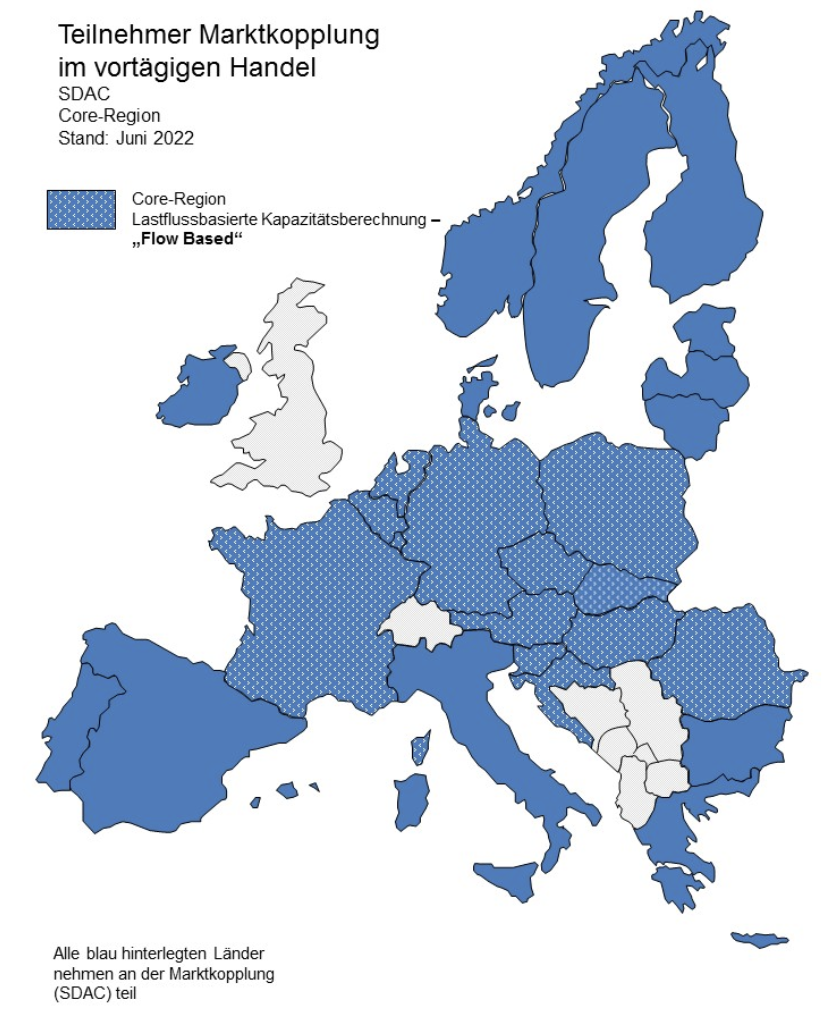
\includegraphics[width=0.5\textwidth]{Graphs/Abbildung1.png}}
    \caption{Karte mit SDAC- und FBMC-Ländern}
    \label{fig:Abbildung1}
\end{figure}

Im Juni 2022 stießen noch weitere osteuropäische Preiszonen hinzu, sodass es nunmehr 12 sind, die das FBMC verwenden (siehe Abbildung~\ref{fig:Abbildung1}).\\
Das Ziel des Market Couplings ist die Angleichung von Preisen. Abbildung~\ref{fig:Abbildung2} und \ref{fig:Abbildung3} zeigen ein Beispiel, das aus dem Paper von \cite{3} stammt, bestehend aus Preiszone A und Preiszone B. Beide Märkte befinden sich jeweils im Gleichgewicht mit einem niedrigeren eigenen Strompreis in Preiszone B und höheren eigenen Preis in Preiszone A. Wenn nun von einer Austausch-Möglichkeit des Stromes ausgegangen wird, wird Strom aus Preiszone B, von Preiszone A aufgekauft, da der Strom in Preiszone B günstiger ist als in A. Das resultiert in einem steigenden Angebot in Preiszone A, was dort den Preis sinken lässt. In Preiszone B hingegen sinkt das Angebot, da nun ein Teil des erzeugten Stromes dort nicht mehr am Markt ist. Der Preis steigt. Dieser Austausch geschieht so lange bis sich beide Preise angeglichen haben. 

\begin{figure}[htbp]
    \centering
    % Erstes Bild
    \begin{minipage}{0.49\textwidth}
        \centering
        \href{https://www.tandfonline.com/doi/abs/10.1080/14697688.2020.1733059}{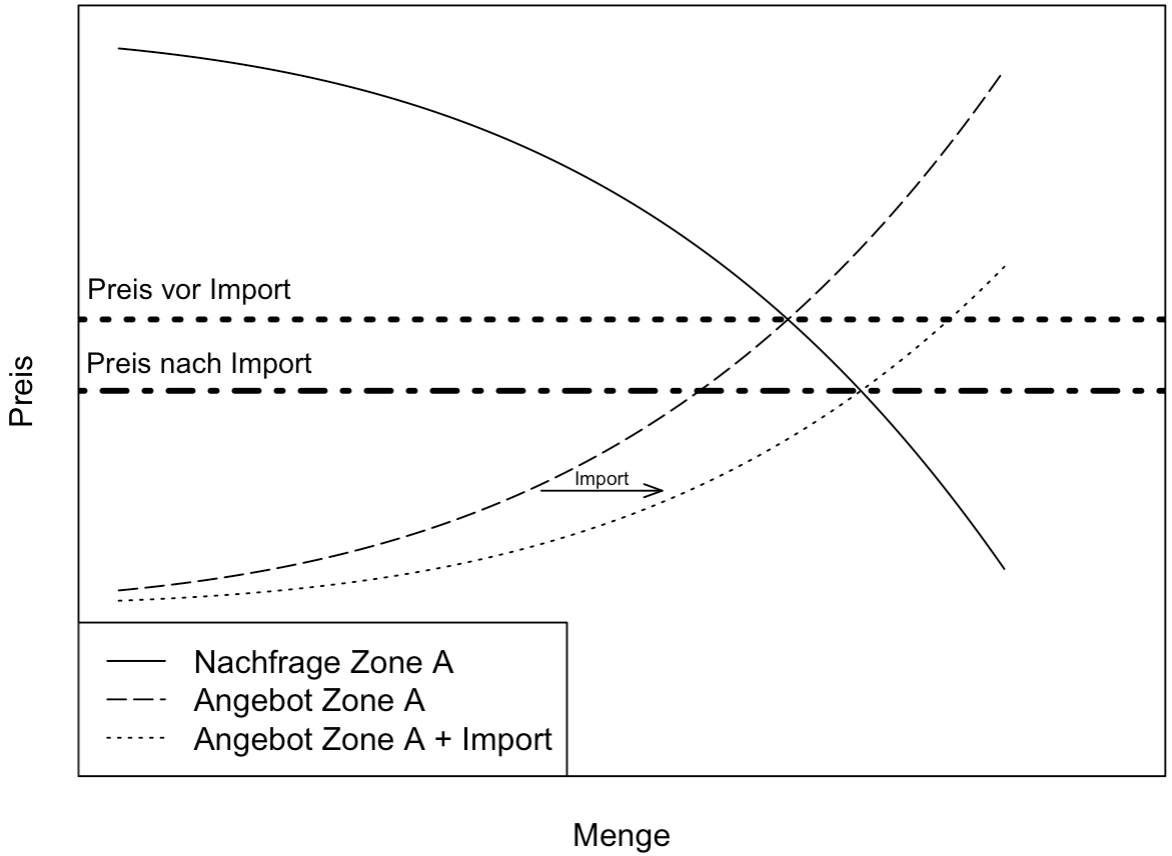
\includegraphics[width=\linewidth]{Graphs/Abbildung2.png}}
        \caption{Preiszone A}    
        \label{fig:Abbildung2}
    \end{minipage}
    \hfill
    % Zweites Bild
    \begin{minipage}{0.49\textwidth}
        \centering
        \href{https://www.tandfonline.com/doi/abs/10.1080/14697688.2020.1733059}{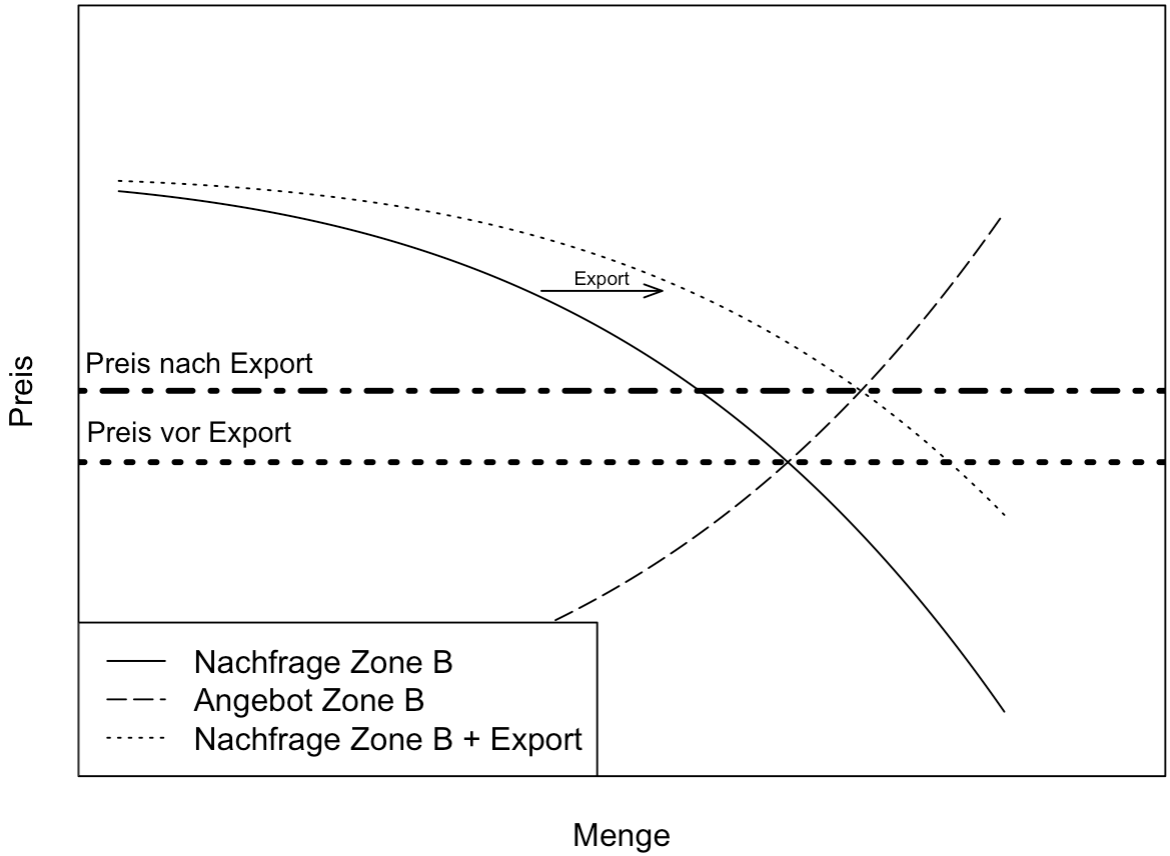
\includegraphics[width=\linewidth]{Graphs/Abbildung3.png}}
        \caption{Preiszone B}        
        \label{fig:Abbildung3}
    \end{minipage}
\end{figure}


\newpage
\subsection{Location Spreads}
\label{sec:Location Spreads}

Wenn der Austausch von Energie zwischen zwei Preiszonen nicht mehr in vollem Umfang möglich ist, gleichen sich die Preise in den Preiszonen nicht an und es entstehen Preisunterschiede (Price Spreads oder auch Location Spreads) durch lokale Preisbildung (\cite{3}). Dieser Austausch wird vor allem dann  behindert, wenn die physikalische Kapazität der grenzüberschreitenden Stromtrassen nicht ausreicht, um den Bedarf an Import oder Export zu decken.\footnote{Weitere seltene Ursachen, die aber im Verlauf der Arbeit nicht weiter untersucht werden, sind z.B. technische Probleme die zum (teilweisen) Ausfall des SDAC führen, wie etwa am 28. Oktober 2023 \cite{ENTSOE_market_report}} \\
Für Marktakteure, insbesondere für Erzeuger erneuerbarer Energien (eE), sind Location Spreads von hoher Relevanz, denn das Wetter und somit auch die Erzeugung von Strom unterliegt großen Schwankungen. In Zeiten hoher Produktion aus Wind oder Photovoltaik kann es zu sehr niedrigen Preisen in Regionen mit hoher Erzeugung kommen, da durch den Merit-Order-Effekt diejenigen Erzeuger von Energien ins Netz einspeisen, die in der Produktion die geringsten Grenzkosten haben (\cite{7}).\\
In Folge dessen wird Strom in eine Preiszone exportiert, die einen höheren Strompreis hat. Sobald allerdings die Interkonnektoren-Kapazität ausgeschöpft ist ist das nicht mehr möglich. Der Strom kann also nicht mehr exportiert werden und flutet nun den heimischen Markt. Der Umstand dass bei gutem Wetter alle Erzeuger von e.E. gleichzeitig Strom in das Netz einspeisen sorgt dafür, dass das Angebot in die Höhe schießt und dadurch der Preis enorm nach unten gedrückt wird. Die Betreiber von Anlagen mit e.E. erhalten also einen niedrigen Preis für ihren Strom. In der Literatur wird zum Beispiel in \cite{7} oder \cite{8} vom Kannibalisationseffekt (Cannibalization Effect) gesprochen. \\
Für Betreiber von e.E.-Anlagen ist es also wichtig sich gegen diese Price Spreads abzusichern. In der Literatur existieren verschiedene Analysen zu Price Spreads. \cite{10} betrachtet Saisonale Trends und Sprünge zwischen zwei Ländern, \cite{12} versucht mit einem Copula Modell und \cite{15} mit Monte-Carlo Simulationen, Abhängigkeiten zwischen extremen Preisen zweier Preiszonen zu erklären. Es gibt auch Untersuchungen von dem Gegenereignis, der Preis Konvergenz. So verwendet \cite{13} etwa lineare Regression und \cite{16} Machine-Learning Ansätze um etwaige Muster zu erkennen\footnote{Das Modell von \cite{16} wird noch von \cite{20} um Einbeziehung von e.E. verfeinert.}.



\newpage
\subsection{Vorstellung relevanter Finanzprodukte}
\label{sec:Vorstellung relevanter Finanzprodukte}
\begin{itemize}

    \item Indizes wie z.B. die von Speedwell Climate  (bspw. Quality Index) \textbf{1, 2}
    \item Je nachdem was am Ende in der Arbeit vorkommt Grundlagen zu diesen Produkten (-> kurze Erklärung zu Optionen, Power Future, Swaps) \textbf{4}
    
\end{itemize}

	\section{Empirische Analyse}
\label{sec:Empirische Analyse}

\subsection{Analyse von Preisdifferenzen}
\label{sec:Analyse von Preisdifferenzen}
\begin{itemize}
    \item Analyse nach Stunden, Off-On-Peak und Monaten 
    \item Ausprobieren gängiger Filter für Saisionalität? 
    \item Nutzen von Regression, Copula Modellen, Monte Carlo? 
\end{itemize}

\subsection{Zusammenhang Location Spreads und Anteil von erneuerbarer Energie}
\label{sec:Zusammenhang Location Spreads und Anteil von erneuerbarer Energie}
\begin{itemize}
    \item Nun Einbeziehung von Residual Load bzw. Solar und Wind einzeln
    \item Verwendung gleicher Methoden (s. o)
\end{itemize}

\subsection{Hedgingmöglichkeiten für Produzenten von Erneuerbarer Energie}
\label{sec:Hedgingmöglichkeiten für Produzenten von Erneuerbarer Energie}
\begin{itemize}
    \item Beispielrechnung mit geeignetem Muster? 
\end{itemize}

        \section{Diskussion der Ergebnisse}
\label{sec:Diskussion der Ergebnisse}

\subsection{Auswirkung und Nutzbarkeit}
\label{sec:Auswirkung und Nutzbarkeit}
Platzhalter

\subsection{Limitationen}
\label{sec:Limitationen}

\begin{itemize}
    \item FBMC nur in 13 Ländern eingesetzt
    \item EE spielen noch längst nicht in allen Ländern eine so große Rolle
    \item Andere Arten von EE nicht betrachtet (Wasserkraft hat z.B. in Österreich einen großen Anteil an EE)
    \item Annahme der unbegrenzten Übertragungskapazität innerhalb einer Zone sinnvoll? \textbf{17}
\end{itemize}


        \section{Fazit und Ausblick}
\label{sec:Fazit und Ausblick}
\begin{itemize}
    \item Kapitel bei 4.3 eingliedern?
    \item Durch Ausbau von Interkonnektoren sinkt Relevanz 
\end{itemize}


	
% Literaturverzeichnis
	\newpage
	%\bibliographystyle{chicago} % Legt den Zitierstil fest.
	%\bibliography{Content/Literaturverzeichnis}
	\printbibliography
% Anhang 
	\newpage
	\appendix % Nummeriert den Anhang mit Buchstaben.
	\section{Anhang}

Platzhalter
	
% Erklärung 
	\newpage\thispagestyle{empty}
	\include{Content/Erklärung_Abschlussarbeit} 
    
\end{document}